% To je predloga za poročila o domačih nalogah pri predmetih, katerih
% nosilec je Blaž Zupan. Seveda lahko tudi dodaš kakšen nov, zanimiv
% in uporaben element, ki ga v tej predlogi (še) ni. Več o LaTeX-u izveš na
% spletu, na primer na http://tobi.oetiker.ch/lshort/lshort.pdf.
%
% To predlogo lahko spremeniš v PDF dokument s pomočjo programa
% pdflatex, ki je del standardne instalacije LaTeX programov.

\documentclass[a4paper,11pt]{article}
\usepackage{a4wide}
\usepackage{fullpage}
\usepackage[utf8x]{inputenc}
\usepackage[slovene]{babel}
\selectlanguage{slovene}
\usepackage[toc,page]{appendix}
\usepackage[pdftex]{graphicx} % za slike
\usepackage{setspace}
\usepackage{color}
\definecolor{light-gray}{gray}{0.95}
\usepackage{listings} % za vključevanje kode
\usepackage{hyperref}
\renewcommand{\baselinestretch}{1.2} % za boljšo berljivost večji razmak
\renewcommand{\appendixpagename}{Priloge}

\lstset{ % nastavitve za izpis kode, sem lahko tudi kaj dodaš/spremeniš
language=Python,
basicstyle=\footnotesize,
basicstyle=\ttfamily\footnotesize\setstretch{1},
backgroundcolor=\color{light-gray},
}

\title{strojno ocenjevanje kratkih odgovorov}
\author{Tomaž Tomažič (63100281)}
\date{\today}

\begin{document}

\maketitle

\section{Uvod}

Cilj naloge je poiskati zanimivo mrežo, jo izrisati in v njej nati skupine
\section{Podatki}

Podatke za gradnjo mreže, sem pobral iz speltne strani Facebook s storitvijo NetGet. V mreži je 160 vozlišč, ki predstavljajo moje prijatelje ~\ref{graf1}. Imam 3 osamelce katere sem za izris ignoriral.

\begin{figure}[htbp]
\begin{center}
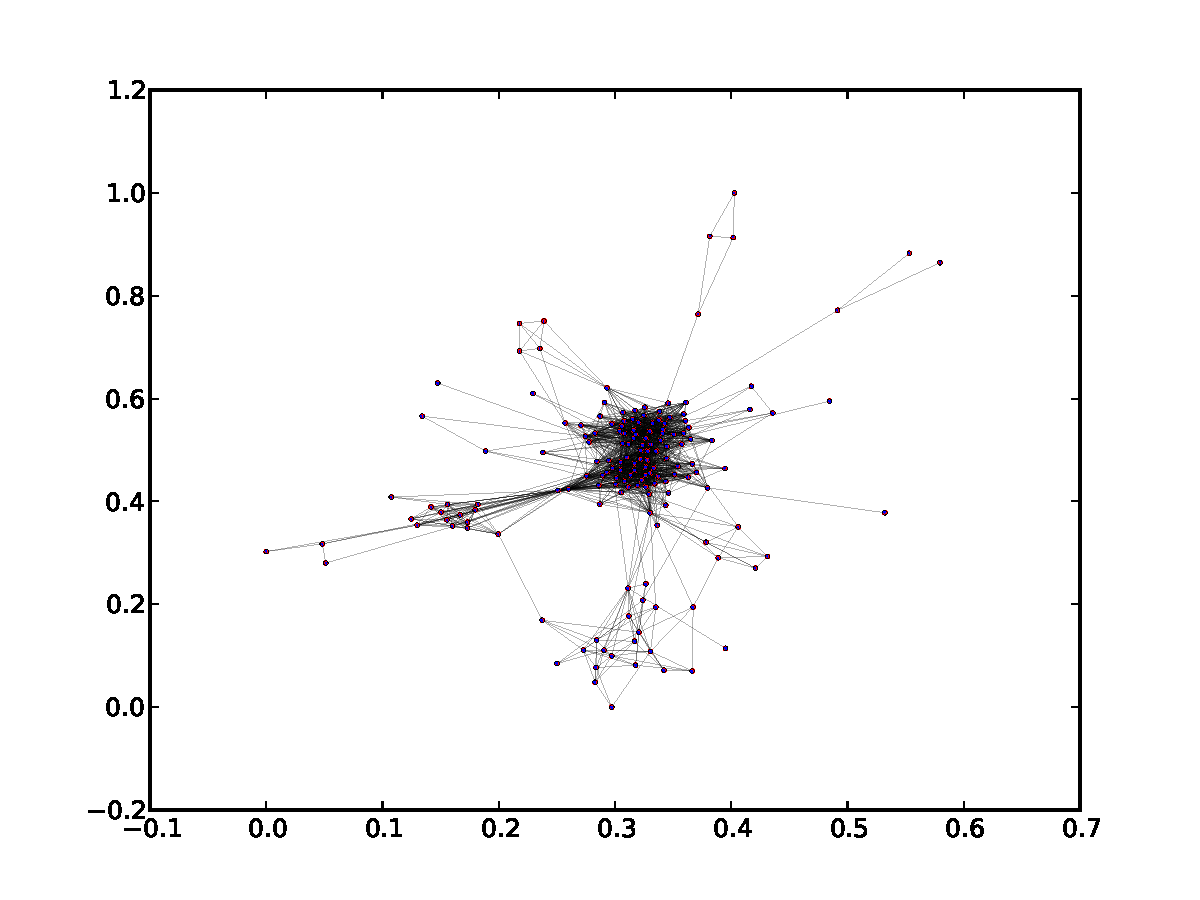
\includegraphics[scale=0.3]{G.pdf}
\caption{Omrežje facebook.}
\label{graf1}
\end{center}
\end{figure}

\section{Metode}

Izračunal sem stopnjo vozlišč v mreži in porazdelitev stopenj  ~\ref{slika1}. 
Postopek za iskanje skupin sem naredil tako, da sem najprej vrstni red vozlišč premešal in v največ 50 iteracijah, vozliščem spreminjal labele, oziroma dokler niso vsa vozlišča pravilno poimenovana. Pravilno poimenovana so takat ko je ime vozlišča enako imenu večine sosedov.

\begin{figure}[htbp]
\begin{center}
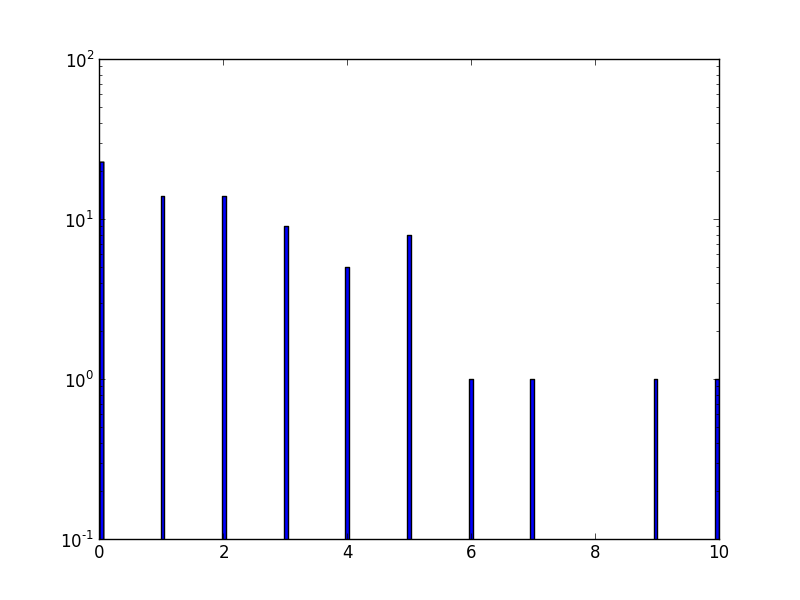
\includegraphics[scale=0.3]{histogram.png}
\caption{Histogram stopenj vozlišč.}
\label{slika1}
\end{center}
\end{figure}

\section{Rezultati}

Odkril sem 7 skupin. Če program večkrat poženem, najde od 6 do 9 skupin. Rezultat ni vedno enak saj je del algoritma naključje. Iz slike je pa  jasno razvidno, da vedno obstajata 2 večji  prevladujoči skupini, v moji mreži.

\section{Izjava o izdelavi domače naloge}
Domačo nalogo in pripadajoče programe sem izdelal sam.

\end{document}

